\section{Gestion des devoirs}

\begin{center}
\scalebox{0.7}{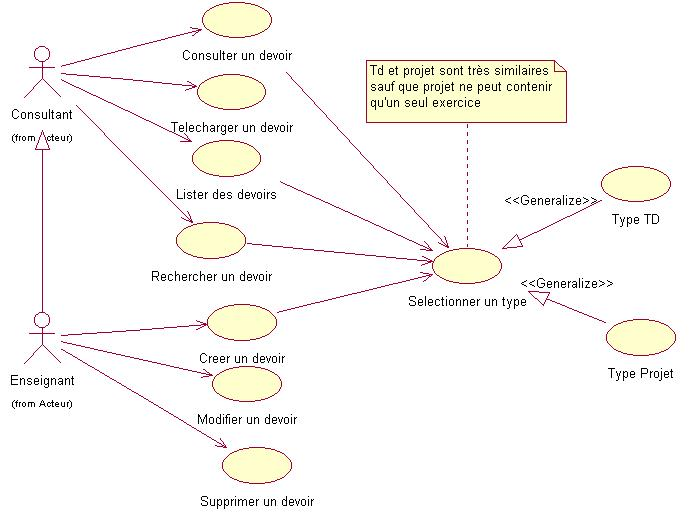
\includegraphics{images/devoir.jpg}}\\
\par{Package Gestion Devoir}
\end{center}

Voici les diff{\'e}rents sc{\'e}narios:\\
\section*{Consultant}

\begin{tabular}{|p{4cm}|c|p{4cm}|p{5cm}|}
\hline
  Fonction & Priorit{\'e} & Qualit{\'e} & Mesure \\
\hline
visualiser un devoir & 5 & Rapide & Permettre un chargement rapide du
  devoir \\
\hline
T{\'e}l{\'e}charger un devoir & 4 & Fiable & Assurer l'int{\'e}gralit{\'e} des donn{\'e}es.\\
\hline
Lister les devoirs & 4 & Rapide et Complet & Permettre de lister
  rapidement les devoirs de l'enseignement souhait{\'e} et assurer le
  listing de tous les devoirs sans omission.\\
\hline
\end{tabular}

\begin{center}
{\'e}chelle de mesure de la priorit{\'e}:

\scalebox{0.5}{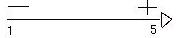
\includegraphics{images/echelle.jpg}}
\end{center}

\begin{itemize}
\item {\bf Visualiser un devoir :}
	\begin{itemize}
	\item Pr{\'e}-requis :Il faut qu'il y ait au moins un devoir de cr{\'e}{\'e}.
	\item Description : Il s{\'e}lectionne successivement les liens lui permettant d'atteindre un projet ou un TD.\\
	Il clique pour le visualiser.
	\item Post-requis : Le devoir s{\'e}lectionn{\'e} est affich{\'e} au format HTML.
	\end{itemize}
		
\item {\bf T{\'e}l{\'e}charger un devoir :}
	\begin{itemize}
	\item Pr{\'e}-requis :Il faut qu'il y ait au moins un devoir de cr{\'e}{\'e}.
	\item Description : Il s{\'e}lectionne successivement les liens lui permettant d'atteindre un projet ou un TD.\\
	Il clique pour le visualiser.
	\item Post-requis : Le devoir s{\'e}lectionn{\'e} est affich{\'e} au format HTML.
	\end{itemize}

\item {\bf Lister des devoirs :}
	\begin{itemize}
	\item Pr{\'e}-requis :Il faut qu'il y ait au moins un devoir de cr{\'e}{\'e}.
	\item Description : Il s{\'e}lectionne successivement les liens lui permettant d'atteindre un projet ou un TD.\\
	Il clique pour le visualiser.
	\item Post-requis : Le devoir s{\'e}lectionn{\'e} est affich{\'e} au format HTML.
	\end{itemize}
			
\item {\bf Rechercher un devoir :}
	\begin{itemize}
	\item Pr{\'e}-requis : Il faut qu'il y ait au moins un devoir de cr{\'e}{\'e}.
	\item Description : Il s{\'e}lectionne successivement les liens lui permettant d'atteindre un projet ou un TD.\\
	Il clique pour le visualiser.
	\item Post-requis :Le devoir s{\'e}lectionn{\'e} est affich{\'e} au format HTML.
	\end{itemize}
\end{itemize}

\section*{Enseignant}

\begin{tabular}{|p{4cm}|c|p{4cm}|p{5cm}|}
\hline
  Fonction & Priorit{\'e} & Qualit{\'e} & Mesure \\
\hline
Cr{\'e}er un devoir & 5 & Rapide et Facile & S{\'e}lection d'exercices dans
  une liste trouv{\'e} gr{\^a}ce aux mots cl{\'e}s ou aux liens par
  l'utilisateur. Ajout simple.\\
\hline
Modifier un devoir & 4 & Rapide et Facile & Permettre un
  ajout/suppression d'un exercice attach{\'e} au devoir tr{\`e}s facilement et
  rapidement (pour la recherche de l'exercice).\\
\hline
Supprimer un devoir & 3 & Fiable & Supprimer uniquement le devoir
  s{\'e}lectionn{\'e}, pas d'incoh{\'e}rence. \\
\hline
\end{tabular}

\begin{center}
{\'e}chelle de mesure de la priorit{\'e}:

\scalebox{0.5}{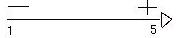
\includegraphics{images/echelle.jpg}}
\end{center}


\begin{itemize}
\item {\bf Cr{\'e}er un devoir :}
	\begin{itemize}
	\item Pr{\'e}-requis : Etre identifi{\'e}.
	\item Description : Il s'identifie avec son login et son mot de passe.\\
	Il s{\'e}lectionne le lien lui permettant de se diriger vers la page de cr{\'e}ation du devoir.\\
	Il s{\'e}lectionne l'enseignement pour lequel le devoir est destin{\'e}.\\
	Il selectionne le type de devoir c'est-{\`a}-dire un projet ou un TD.\\
	Il s{\'e}lectionne un ou plusieurs exercices dans une liste d'exercices pr{\'e}-enregistr{\'e}s ou il le(s) importe.\\
	Il choisit pour chaque exercice son emplacement dans la hierarchie.\\
	Remarque: Un projet ne peut contenir qu'un seul exercice.\\  
	Il valide sa s{\'e}lection.
	\item Post-requis : Un nouveau devoir est enregistr{\'e} dans la liste des devoirs disponibles (Projet ou TD).
	\end{itemize}

\item {\bf Modifier devoir :}
	\begin{itemize}
	\item Pr{\'e}-requis : Etre identifi{\'e}.\\
	Il faut qu'au moins un projet soit enregistr{\'e}.
	\item Description : Il s'identifie avec son login et son mot de passe.\\
	Il s{\'e}lectionne le lien lui permettant de se diriger vers la page des devoirs dans un enseignement.\\
	Il peut d{\'e}placer le devoir dans un autre enseignement. \\
	Il peut modifier le devoir par un autre exercice de type projet dans la liste des exercices.\\
	Il valide sa s{\'e}lection.
	\item : Avertissement : Si l'enseignant qui modifie le projet n'est pas son cr{\'e}ateur, alors une sauvegarde de l'{\'e}l{\'e}ment modifi{\'e} sera effectu{\'e} pour avoir la possibilit{\'e} de revenir sur cette modification.
	\item Post-requis : Le devoir est modifi{\'e} dans la liste des devoir disponibles.
	\end{itemize}

\item {\bf Supprimer devoir :}
	\begin{itemize}
	\item Pr{\'e}-requis : Etre identifi{\'e}.\\
	Il faut qu'au moins un devoir soit enregistr{\'e}.\\
	Il doit {\^e}tre le cr{\'e}ateur du devoir.
	\item Description : Il s'identifie avec son login et son mot de passe.\\
	Il s{\'e}lectionne successivement les liens lui permettant de se diriger vers la page de modification de devoir.\\
	Il peut demander la suppression du devoir. Il valide sa demande.
	\item : Avertissement : Un enseignant ne peut pas supprimer un devoir ne lui appartenant pas.
	\item : Post-requis : le devoir est supprim{\'e} (s'il est son cr{\'e}ateur).\\
	\end{itemize}
\end{itemize}
